\chapter{Midterm 1}

The first chapter of the project report contains background information about the problem, the associated domain and the impact the problem has on the identified domain. 
Also, when knowing the domain, one could establish target groups and perform customer validation in order to justify the relevance of the problem and the need for the project itself. \cite{chicago}

Also, it is important to represent the project in a comparative analysis in relation to other analogs. 
By doing this, the project team can emphasize what the analogs lack and what the new solution could improve.


\section{Problem Description and Problem Analysis}

The origin of the project is the problem itself. 
Naturally, the project team should continue the work on the project by building their way around the problem description. 
A good description of the problem forms that foundation of the other aspects and allows the team to do progress.

Any problem has it's impact in the scope of one or multiple domains.
It is important to identify this scope so that the problem could be analyzed and see what is the impact over the domain. 
Having that in place, the project team can come up with a concept for a solution to the analyzed problem. \cite{chicago}


\addcontentsline{toc}{section}{Solution Proposal}
\section{Solution Proposal}

The next step after describing and analyzing the problem is to create a concept for the proposed solution. 
The concept is just an initial vector for the rest of the project. 
It should be simple and on point, giving an overview on what you intend to design.
\vspace{0.5cm}

{ \centering 
\includegraphics[width=\textwidth]{images/concept.png} }

The solution concept should be represented by a project name and the objectives that the project teams has.
Basically the objectives would help with the definition of the requirements and also can help other people to understand the idea behind the project.

As time is limited and there are lot's of new things to learn and use, probably the project teams will not get all the things right the first time.
The first iteration through the requirements for the 1st midterm will be presented at the evaluation and the teams should be confident on what has been done.
\vspace{0.5cm}

{ \centering 
\includegraphics[width=\textwidth]{images/before.png} }

All the gathered information should be taken as the base for the work that comes next. 
Also, the feedback from the mentors should be considered in order to fix the issues if any, and to polish what has been done so far.
With that in mind, iteration after iteration, the concept takes shape and the project covers more of the initial requirements.

{ \centering 
\includegraphics[width=\textwidth]{images/after.png} }


\section{Target Group and Customer Validation}

The target group represents an audience that is identified as potential users of a product. 
Basically the individuals from a target group have something in common which can be things like age, occupation, hobbies etc., or maybe they are just bothered by the same problem.

The target group should be presented in this section and, if applicable, any classification of the target group into sub-groups should be enlisted as well. 
This can be done in list, tabular forms or even plain text.

{ \centering 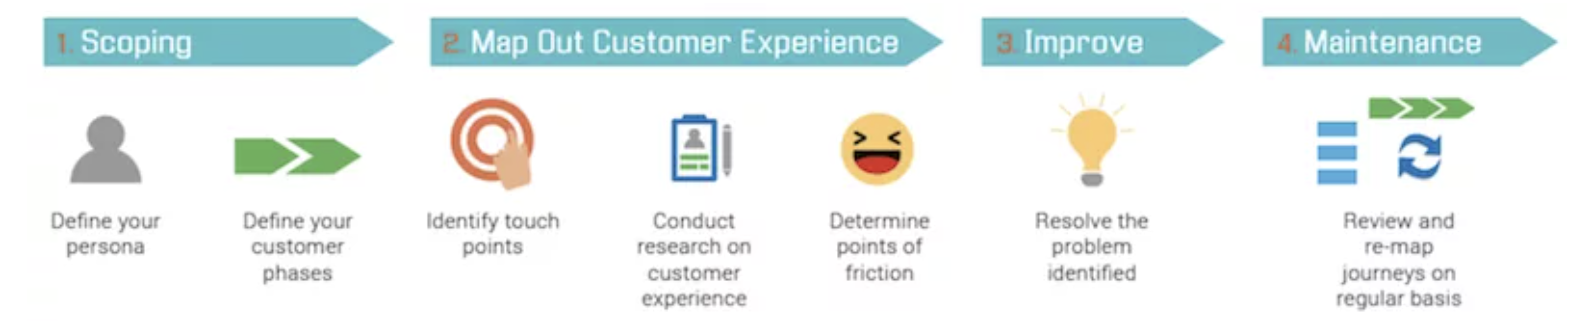
\includegraphics[width=\textwidth]{images/problem_analysis.png} }


\section{Comparative Analysis}

Here goes your comparative analysis..


% \section{Domain Analysis Conclusions}
% \begin{enumerate}
%     \item The current chapter presented a thorough domain analysis and customer validation for project X.
%     \item While performing the domain analysis the identified target groups are the following: A, B, C.
% \end{enumerate}